\documentclass[a4paper,12pt]{article}

% Ngôn ngữ và mã hóa
\usepackage[utf8]{inputenc}
\usepackage[T5]{fontenc}
\usepackage[vietnamese]{babel}

% Lề trang và giãn dòng
\usepackage[margin=1in]{geometry}
\usepackage{setspace}
\usepackage{indentfirst}
\setstretch{1.15}

% Toán học
\usepackage{amsmath,amssymb}
\usepackage{latexsym}

% Bảng và hình
\usepackage{graphicx}
\usepackage{array}
\usepackage{tabularx}
\usepackage{booktabs}
\usepackage{multirow}
\usepackage{makecell}
\usepackage{colortbl}
\usepackage{subcaption}
\usepackage{float}
\usepackage{caption}
\usepackage{rotating}
\usepackage{multicol}

% Danh sách, thuật toán, khung nội dung và mã nguồn
\usepackage{enumerate}
\usepackage{enumitem}
\usepackage[lined,boxed,commentsnumbered]{algorithm2e}
\usepackage[most]{tcolorbox}
\usepackage{listings}
\usepackage{xcolor}
\usepackage{fancyvrb}
\usepackage{verbatim}

% Các tiện ích khác
\usepackage{pgfgantt}
\usepackage{tikz}
\usepackage{afterpage}
\usepackage{lastpage}
\usepackage{fancyhdr}
\usepackage{hyperref}

% Thiết lập siêu liên kết
\hypersetup{
    colorlinks=true,
    linkcolor=blue,
    citecolor=blue,
    urlcolor=blue
}

% Màu cho mã nguồn
\definecolor{codegreen}{rgb}{0,0.6,0}
\definecolor{codegray}{rgb}{0.5,0.5,0.5}
\definecolor{codeorange}{rgb}{1,0.49,0}
\definecolor{backcolour}{rgb}{0.95,0.95,0.96}
\definecolor{pink}{RGB}{255, 121, 198}
\definecolor{red}{RGB}{255, 85, 85}

\lstdefinestyle{mystyle}{
    language=Matlab,
    basicstyle=\ttfamily\small,
    numbers=left,
    numberstyle=\tiny\color{codegray},
    stepnumber=1,
    numbersep=5pt,
    showstringspaces=false,
    tabsize=2,
    breaklines=true,
    breakatwhitespace=false,
    captionpos=b,
    commentstyle=\color{codegreen},
    keywordstyle=\color{pink},
    stringstyle=\color{red},
    inputencoding=utf8,
    extendedchars=true
}
\lstset{style=mystyle}

% Môi trường định lý
\newtheorem{theorem}{{\bf Định lý}}
\newtheorem{property}{{\bf Tính chất}}
\newtheorem{proposition}{{\bf Mệnh đề}}
\newtheorem{corollary}[proposition]{{\bf Hệ quả}}
\newtheorem{lemma}[proposition]{{\bf Bổ đề}}

% Tên hiển thị tiếng Việt
\AtBeginDocument{\renewcommand*\contentsname{Mục lục}}
\AtBeginDocument{\renewcommand*\refname{Tài liệu tham khảo}}

% Đầu trang và chân trang
\setlength{\headheight}{40pt}
\pagestyle{fancy}
\fancyhead{}
\fancyhead[L]{
    \begin{tabular}{rl}
        \begin{picture}(25,15)(0,0)
            \put(0,-8){
\includegraphics[width=8mm,height=8mm]{uploads/HCMUT.png}}
        \end{picture}&
        \begin{tabular}{l}
            \textbf{\ttfamily Trường Đại học Bách khoa, ĐHQG-TPHCM}\\
            \textbf{\ttfamily Khoa Khoa học và Kỹ thuật Máy tính}
        \end{tabular}
    \end{tabular}
}
\fancyhead[R]{\ttfamily \textit{Dữ liệu lớn - CO5135}}
\fancyfoot{}
\fancyfoot[L]{\scriptsize\ttfamily Báo cáo Dữ liêu lớn - Học kỳ 2 - Năm học 2025-2026}
\fancyfoot[R]{\scriptsize\ttfamily Trang \thepage/\pageref{LastPage}}
\renewcommand{\headrulewidth}{0.3pt}
\renewcommand{\footrulewidth}{0.3pt}

% Độ sâu mục lục
\setcounter{secnumdepth}{4}
\setcounter{tocdepth}{3}
\makeatletter
\newcounter{subsubsubsection}[subsubsection]
\renewcommand\thesubsubsubsection{\thesubsubsection.\@alph\c@subsubsubsection}
\newcommand\subsubsubsection{\@startsection{subsubsubsection}{4}{\z@}%
    {-3.25ex\@plus -1ex \@minus -.2ex}%
    {1.5ex \@plus .2ex}%
    {\normalfont\normalsize\bfseries}}
\newcommand*\l@subsubsubsection{\@dottedtocline{3}{10.0em}{4.1em}}
\newcommand*{\subsubsubsectionmark}[1]{}
\makeatother

\begin{document}

\pagenumbering{gobble}
\hypersetup{pageanchor=false}
\begin{titlepage}
\begin{center}
ĐẠI HỌC QUỐC GIA THÀNH PHỐ HỒ CHÍ MINH\\
TRƯỜNG ĐẠI HỌC BÁCH KHOA\\
KHOA KHOA HỌC VÀ KỸ THUẬT MÁY TÍNH
\end{center}

\vspace{1cm}

\begin{figure}[h!]
\centering

\includegraphics[width=3cm]{uploads/HCMUT.png}
\end{figure}

\vspace{1cm}

\begin{center}
\begin{tabular}{c}
\multicolumn{1}{l}{\textbf{{\Large Dữ liêu lớn - CO5135}}}\\
~~\\
\hline
\\
\multicolumn{1}{l}{\textbf{{\Large Mini-project}}}\\
\\
\textbf{{\huge Đề tài:}}\\
\\
\multicolumn{1}{c}{
\begin{minipage}{0.92\textwidth}
\centering
\textbf{{\LARGE Phát hiện video độc hại trên các nền tảng phát trực tuyến dựa trên học giám sát yếu và gán nhãn giả.}}
\end{minipage}
}\\
\\
\hline
\end{tabular}
\end{center}

\vspace{3cm}

\begin{table}[h]
\begin{tabular}{rrl}
\hspace{5cm} & Giảng viên hướng dẫn: & \textit{PGS.TS Thoại Nam}\\
\\
& Học viên: & \textit{Nguyễn Duy Hòa - 2570782}\\
& & \textit{Nguyễn Lê Gia Hinh - 2570781}\\
% & & \textit{Họ tên - Mã số sinh viên}\\
\end{tabular}
\normalsize
\end{table}

\begin{center}
{\footnotesize THÀNH PHỐ HỒ CHÍ MINH, THÁNG 6/2026}
\end{center}
\end{titlepage}

\hypersetup{pageanchor=true}
\pagenumbering{roman}
\newpage
\tableofcontents
\newpage
\pagenumbering{arabic}


\section{Danh sách thành viên và phân công nhiệm vụ}

\begin{table}[H]
\centering
\scriptsize
\renewcommand{\arraystretch}{1.5}
\begin{tabular}{|>{\centering\arraybackslash}m{0.8cm}|>{\centering\arraybackslash}m{3.4cm}|>{\centering\arraybackslash}m{1.9cm}|>{\centering\arraybackslash}m{4.4cm}|>{\centering\arraybackslash}m{2.4cm}|}
\hline
\textbf{STT} & \textbf{Họ và tên} & \textbf{Mã số sinh viên} & \textbf{Nhiệm vụ được phân công} & \textbf{Tỷ lệ đóng góp}\\
\hline
1 &  &  &  &  \\
\hline
2 &  &  &  &  \\
\hline
3 &  &  &  &  \\
\hline
\end{tabular}
\normalsize
\end{table}


\clearpage

\section{Introduction}

\subsection{Background and Motivation}

Online streaming platforms host a large and constantly growing amount of user-generated video content. This scale creates a difficult moderation problem: harmful videos can spread quickly, while manual review is costly, slow, and difficult to apply consistently across large collections of content. A practical detection system therefore needs to support moderation triage by identifying videos that are likely to be harmful and should be prioritized for further review.

This project focuses on harmful video detection using text signals that are commonly associated with online videos: the title, description, and transcript. A text-first design is intentionally chosen for the first version because these fields are easier to process in a local batch pipeline than thumbnails, video frames, or audio streams. Text features also provide a strong starting point for a Big Data project because they allow the system to emphasize ingestion, schema normalization, scalable data processing, model comparison, and reproducible evaluation.

The project is framed for streaming platforms in general, but the experimental evaluation is limited to a local YouTube-derived MetaHarm dataset. Therefore, the main claim of the project is not that the trained model is already proven across all platforms. Instead, the project demonstrates a generalizable pipeline design for harmful video detection, with clear data contracts, auditability, weak supervision, pseudo-labeling, and a small demo service.

\begin{figure}[H]
\centering
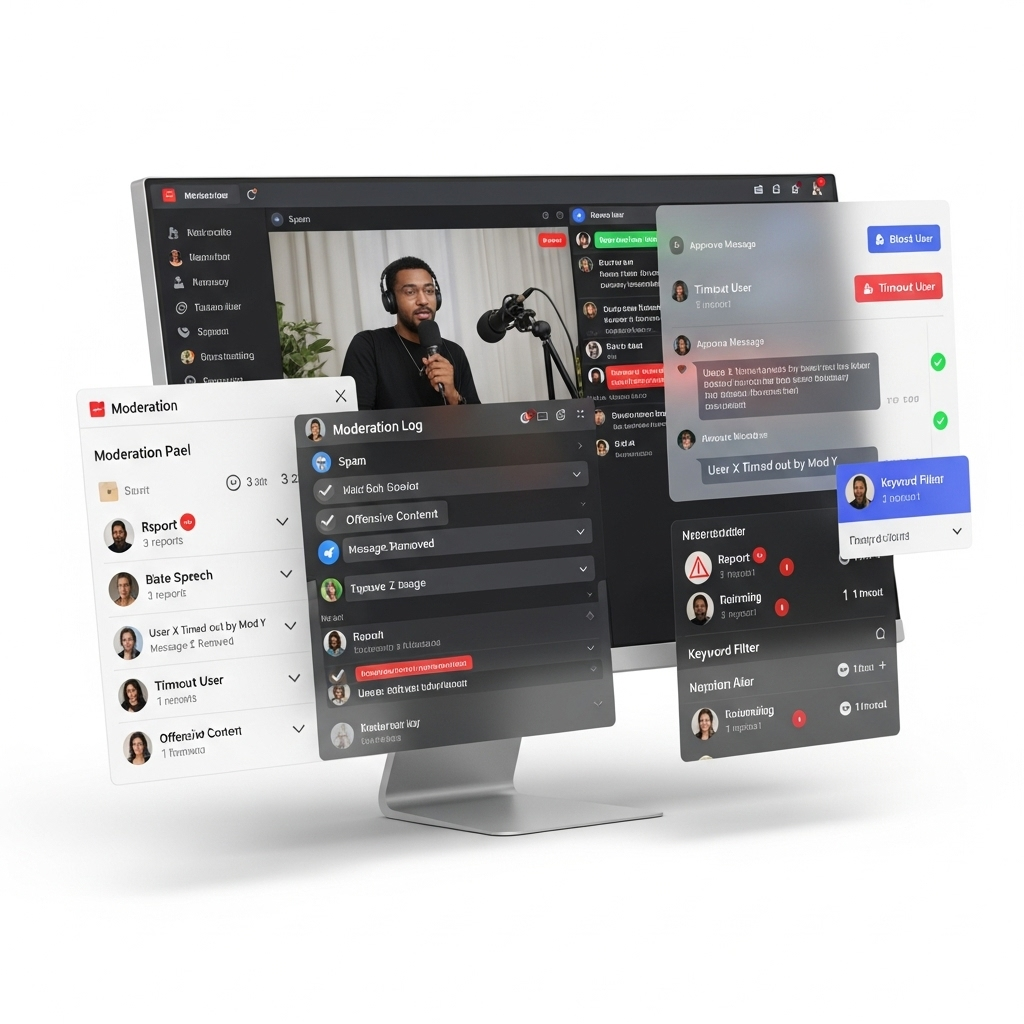
\includegraphics[width=0.88\textwidth]{uploads/intro_streaming_content_moderation.png}
\caption{Conceptual content moderation workflow for streaming platforms. The figure illustrates the broader moderation context; this project implements an offline, text-first batch pipeline rather than live stream deactivation or image-frame moderation.}
\label{fig:introduction-content-moderation-context}
\end{figure}

\subsection{Problem Statement}

The core problem is binary harmful video detection. Given a video's available text fields, the system predicts whether the video should be considered harmful or harmless. The input contract is intentionally simple:

\begin{itemize}
    \item \textbf{Title}: the video title text.
    \item \textbf{Description}: the video description text.
    \item \textbf{Transcript}: the available speech transcript or extracted text transcript.
\end{itemize}

The output of the core classifier is a harmful probability and a binary decision. In the demo API, this probability is also mapped into a risk band: low, medium, or high. This output is intended as a decision-support signal for review prioritization, not as a complete automated moderation decision.

The project does not use channel identity, view count, duration, thumbnails, image frames, or live streaming signals in the core classifier. Channel identity may introduce creator leakage, while view count and duration are not consistently available in all labeled sources. Visual and audio features are useful future extensions, but they increase setup complexity and are not required for the first stable version of the pipeline.

\subsection{Project Objectives}

The project has the following objectives:

\begin{itemize}
    \item Build a reproducible local batch pipeline for harmful video detection.
    \item Organize raw, cleaned, and modeling-ready data using bronze, silver, and gold data layers.
    \item Normalize heterogeneous spreadsheets and CSV files into a unified schema.
    \item Preserve audit information for dropped rows, duplicate records, canonical text selection, and label conflicts.
    \item Use domain expert labels as the primary supervised ground truth.
    \item Train an expert-only baseline model for binary harmful vs harmless classification.
    \item Use GPT-4-Turbo and crowdworker labels as weak supervision sources.
    \item Run one round of pseudo-labeling on the unlabeled pool using strict confidence thresholds.
    \item Compare expert-only, expert plus weak supervision, and expert plus weak supervision plus pseudo-labeling models using the same validation and test splits.
    \item Expose the selected binary model through a small local prediction API.
\end{itemize}

\subsection{Dataset and Scope}

The experimental dataset contains multiple label sources, including domain expert annotations, GPT-4-Turbo annotations, crowdworker annotations, agreement subsets, and an unlabeled pool. These sources are derived from YouTube data in the MetaHarm setting. Because the sources differ in structure, quality, and coverage, the project treats data engineering as a central part of the solution rather than a preprocessing afterthought.

The current scope is limited to binary harmful vs harmless detection. Six-category harm classification is kept as a phase-two extension after the binary system is stable. The project is also text-first: thumbnails, frame-level image features, audio modeling, live scraping, and real-time event streaming are excluded from the completed system. This boundary makes the project more reproducible and keeps the main contribution focused on data processing, weak supervision, pseudo-labeling, and reliable model evaluation.

\subsection{Main Contributions}

The main contributions of this project are:

\begin{itemize}
    \item A local single-node data pipeline that converts raw annotation files and unlabeled text records into modeling-ready datasets.
    \item A bronze, silver, and gold data organization pattern for preserving raw data, enforcing a common schema, and building canonical training tables.
    \item A canonical text selection rule that keeps the longest non-empty title, description, and transcript for each duplicated video identifier.
    \item Audit logic that records dropped rows, duplicate handling, source-level cleanup, and label conflicts.
    \item An annotator agreement analysis comparing domain expert, GPT-4-Turbo, and crowdworker binary labels.
    \item A TF-IDF logistic regression baseline trained only on domain expert labels.
    \item A weak-supervision extension that estimates source reliability and accepts only confident weak labels.
    \item A pseudo-labeling experiment that uses high-confidence predictions from the unlabeled pool and applies a validation-based fallback rule.
    \item A demo API that returns a harmful probability, binary prediction, risk band, and model version for short text inputs.
\end{itemize}

\subsection{Report Organization}

The remainder of the report is organized as follows. Section 3 presents the theoretical background, including harmful video detection, text-first modeling, weak supervision, pseudo-labeling, TF-IDF logistic regression, and evaluation metrics. Section 4 describes the implementation methodology and experimental results, including the data pipeline, agreement analysis, model comparison, pseudo-labeling outcome, error analysis, and demo API. Section 5 summarizes the findings, discusses limitations, and proposes future work.


\clearpage

\section{Cơ sở lý thuyết}

\subsection{Phát hiện video độc hại}

Phát hiện video độc hại là một bài toán phân loại nội dung, trong đó hệ thống ước lượng liệu một video có chứa hoặc cổ xúy nội dung không an toàn, lạm dụng, gây hiểu lầm, bóc lột hoặc vi phạm chính sách hay không. Trong bối cảnh kiểm duyệt thực tế, mô hình loại này thường không được kỳ vọng tự đưa ra quyết định thực thi cuối cùng. Thay vào đó, mô hình có thể hỗ trợ phân loại ưu tiên bằng cách xác định những nội dung cần được rà soát kỹ hơn.

Đề tài này mô hình hóa nhiệm vụ cốt lõi dưới dạng phân loại nhị phân:

\begin{equation}
    y =
    \begin{cases}
        1, & \text{nếu video độc hại},\\
        0, & \text{nếu video không độc hại}.
    \end{cases}
\end{equation}

Cách phát biểu nhị phân được chọn làm sản phẩm chính vì đơn giản hơn, dễ đánh giá một cách đáng tin cậy hơn và phù hợp hơn để xây dựng một pipeline dữ liệu đầu cuối ổn định. Một cách phát biểu đa nhãn chi tiết hơn có thể được áp dụng khi cần gán video vào các loại tác hại cụ thể. Trong đề tài này, sáu nhãn loại \texttt{IH}, \texttt{HH}, \texttt{CB}, \texttt{ADD}, \texttt{SXL} và \texttt{PH} được xem là phần mở rộng giai đoạn hai, không thuộc hệ thống cốt lõi đã hoàn thiện.

\subsection{Thiết kế đặc trưng ưu tiên văn bản}

Video có thể chứa nhiều nguồn thông tin khác nhau, bao gồm khung hình, âm thanh, siêu dữ liệu, bình luận, tín hiệu tương tác và phần mô tả bằng văn bản. Đề tài này bắt đầu bằng một thiết kế ưu tiên văn bản (text-first). Đầu vào của mô hình được giới hạn trong ba trường:

\begin{itemize}
    \item \textbf{Tiêu đề}: phần tóm tắt ngắn được viết cho người xem.
    \item \textbf{Mô tả}: phần văn bản ngữ cảnh dài hơn đi kèm video.
    \item \textbf{Bản ghi lời nói}: nội dung nói được chuyển thành văn bản khi có sẵn.
\end{itemize}

Văn bản đầu vào hợp nhất cho mô hình có thể được biểu diễn như sau:

\begin{verbatim}
model_text = normalize(title)
           + normalize(description)
           + normalize(transcript)
\end{verbatim}

Các trường rỗng được bỏ qua và khoảng trắng được chuẩn hóa trước khi đưa vào mô hình. Thiết kế này giúp hệ thống có khả năng tái lập và giảm phụ thuộc vào các công cụ bên ngoài để trích xuất ảnh, xử lý âm thanh hoặc thu thập dữ liệu theo đặc thù nền tảng. Thiết kế này cũng giảm rủi ro rò rỉ dữ liệu bằng cách loại trừ các đặc trưng như danh tính kênh, số lượt xem và thời lượng. Danh tính kênh có thể khiến mô hình học các mẫu ở cấp người tạo nội dung thay vì tín hiệu ở cấp nội dung, trong khi các trường về độ phổ biến và thời lượng không có mặt nhất quán trên tất cả các nguồn có nhãn.

\subsection{Các tầng dữ liệu Bronze, Silver và Gold}

Học máy đáng tin cậy phụ thuộc vào kỹ thuật dữ liệu đáng tin cậy. Đề tài sử dụng mô hình tổ chức dữ liệu ba tầng: bronze, silver và gold. Mỗi tầng giữ một vai trò riêng trong pipeline.

\begin{table}[H]
\centering
\renewcommand{\arraystretch}{1.35}
\begin{tabularx}{\textwidth}{|>{\raggedright\arraybackslash}p{2.2cm}|>{\raggedright\arraybackslash}X|}
\hline
\textbf{Tầng} & \textbf{Mục đích} \\
\hline
Bronze & Bảo toàn các bản ghi nguồn thô và siêu dữ liệu nhập dữ liệu gần nhất có thể với tệp gốc. \\
\hline
Silver & Chuẩn hóa các nguồn không đồng nhất thành một lược đồ ở cấp dòng với tên trường, nhãn, trường văn bản và cờ chất lượng nhất quán. \\
\hline
Gold & Xây dựng các bảng sẵn sàng cho mô hình, trường văn bản chuẩn hóa, tập train/validation/test, tóm tắt đồng thuận và kết quả kiểm toán. \\
\hline
\end{tabularx}
\caption{Vai trò khái niệm của các tầng dữ liệu bronze, silver và gold.}
\label{tab:theory-data-layers}
\end{table}

Tầng bronze hỗ trợ khả năng truy vết vì bảo toàn nội dung đã được nhập. Tầng silver hỗ trợ tính nhất quán vì mọi nguồn đều được chuyển đổi về cùng một lược đồ. Tầng gold hỗ trợ mô hình hóa vì tạo ra một bản ghi chuẩn hóa cho mỗi mã định danh video và chuẩn bị đầu vào sạch cho huấn luyện cũng như đánh giá.

Thiết kế phân tầng đặc biệt hữu ích khi các tệp nguồn không đồng nhất. Trong đề tài này, dữ liệu bao gồm bảng tính, tệp CSV, nhiều nguồn chú thích, tệp trùng lặp, mã định danh video bị thiếu, tên cột không nhất quán và mức độ sẵn có của văn bản khác nhau. Pipeline phân tầng giúp các vấn đề này trở nên quan sát được thay vì bị che giấu bên trong mã huấn luyện mô hình.

\subsection{Giám sát yếu}

Giám sát yếu (weak supervision) là một chiến lược học sử dụng các nguồn nhãn chưa hoàn hảo để tăng lượng dữ liệu huấn luyện. Các nhãn này có thể rẻ hơn, nhiễu hơn hoặc ít có thẩm quyền hơn nhãn chuyên gia. Trong đề tài này, nhãn của chuyên gia lĩnh vực được xem là ground truth chính, trong khi nhãn của GPT-4-Turbo và crowdworker được xem là các nguồn yếu.

Ý tưởng cốt lõi không phải là tin tưởng mọi nhãn yếu như nhau. Thay vào đó, hệ thống ước lượng độ tin cậy của từng nguồn yếu bằng cách so sánh nguồn đó với nhãn chuyên gia lĩnh vực trên phần giao nhau thuộc tập huấn luyện có nhãn chuyên gia:

\begin{equation}
    r_s = \frac{\#\text{số lần nguồn }s\text{ đồng thuận với chuyên gia lĩnh vực}}{\#\text{số mẫu huấn luyện giao nhau}}.
\end{equation}

Các độ tin cậy sau đó được chuẩn hóa thành trọng số:

\begin{equation}
    w_{\text{GPT}} =
    \frac{r_{\text{GPT}}}{r_{\text{GPT}} + r_{\text{Crowd}}},
    \qquad
    w_{\text{Crowd}} =
    \frac{r_{\text{Crowd}}}{r_{\text{GPT}} + r_{\text{Crowd}}}.
\end{equation}

Đối với một video có các nhãn yếu khả dụng, xác suất độc hại yếu được tính như một trung bình có trọng số:

\begin{equation}
    p_{\text{weak}} =
    \frac{\sum_{s \in S} w_s y_s}{\sum_{s \in S} w_s},
\end{equation}

trong đó \(S\) là tập các nguồn yếu khả dụng và \(y_s \in \{0,1\}\) là nhãn nhị phân từ nguồn \(s\). Sau đó, hệ thống áp dụng một quy tắc chấp nhận thận trọng:

\begin{verbatim}
if weak_p >= 0.75:
    accept as harmful
elif weak_p <= 0.25:
    accept as harmless
else:
    abstain
\end{verbatim}

Các nhãn yếu được chấp nhận sẽ nhận trọng số mẫu dựa trên độ tự tin:

\begin{equation}
    \text{trọng số mẫu} = 0.5 + |p_{\text{weak}} - 0.5|.
\end{equation}

Quy tắc này gán trọng số cao hơn cho các nhãn yếu nằm xa vùng bất định và trọng số thấp hơn cho các nhãn gần biên quyết định.

\subsection{Gán nhãn giả}

Gán nhãn giả (pseudo-labeling) là một phương pháp tự huấn luyện, trong đó mô hình đã huấn luyện được dùng để gán nhãn cho các mẫu chưa có nhãn. Những nhãn được sinh tự động này chỉ được thêm vào tập huấn luyện nếu thỏa mãn các yêu cầu về độ tin cậy. Mục tiêu là khai thác tập chưa gán nhãn mà không cần chú thích thủ công cho từng mẫu.

Trong đề tài này, gán nhãn giả được thiết kế một cách thận trọng. Trước hết, mô hình giám sát yếu tốt nhất được dùng để chấm điểm các video chưa gán nhãn. Một nhãn giả chỉ được chấp nhận nếu mẫu có đủ văn bản và xác suất độc hại đã hiệu chỉnh nằm rất gần 0 hoặc 1:

\begin{verbatim}
if token_count >= 30 and (p_harmful >= 0.95 or p_harmful <= 0.05):
    accept pseudo-label
else:
    discard
\end{verbatim}

Tất cả nhãn giả được chấp nhận nhận trọng số mẫu cố định bằng 0.5. Mô hình được huấn luyện lại một lần duy nhất và quá trình tự huấn luyện dừng lại sau vòng đó. Cách làm này ngăn các vòng phản hồi không kiểm soát, trong đó lỗi của mô hình có thể bị củng cố lặp đi lặp lại.

Quy tắc cuối cùng cho gán nhãn giả dựa trên tập validation. Mô hình có nhãn giả chỉ được giữ lại nếu không làm giảm macro-F1 trên validation hoặc recall của lớp độc hại so với mô hình giám sát yếu. Quy tắc này quan trọng vì gán nhãn giả có thể làm tăng kích thước tập huấn luyện nhưng vẫn làm giảm chất lượng mô hình nếu các nhãn được chấp nhận bị lệch hoặc sai.

\begin{figure}[H]
\centering
\resizebox{0.98\textwidth}{!}{
\begin{tikzpicture}[
    box/.style={draw, rounded corners, align=center, minimum width=3.3cm, minimum height=1.05cm, font=\small},
    source/.style={box, fill=blue!10},
    model/.style={box, fill=green!10},
    decision/.style={box, fill=orange!15},
    arrow/.style={->, thick}
]
\node[source] at (0,2.4) (expert) {Nhãn chuyên gia\\lĩnh vực};
\node[source] at (0,0.8) (weak) {Nguồn yếu\\GPT và crowd};
\node[source] at (0,-0.8) (unlabeled) {Tập văn bản\\chưa gán nhãn};

\node[model] at (4.2,2.4) (baseline) {Mô hình nền\\chỉ chuyên gia};
\node[model] at (4.2,0.8) (weakmodel) {Chuyên gia +\\giám sát yếu};
\node[model] at (4.2,-0.8) (pseudomodel) {Chuyên gia + yếu +\\gán nhãn giả};
\node[decision] at (8.5,0.8) (selection) {Chọn mô hình\\theo validation};

\draw[arrow] (expert) -- (baseline);
\draw[arrow] (expert) -- (weakmodel);
\draw[arrow] (weak) -- node[above, font=\scriptsize] {nhãn có trọng số} (weakmodel);
\draw[arrow] (weakmodel) -- node[above, font=\scriptsize] {chấm điểm văn bản chưa gán nhãn} (pseudomodel);
\draw[arrow] (unlabeled) -- node[below, font=\scriptsize] {nhãn độ tin cậy cao} (pseudomodel);
\draw[arrow] (baseline) -- (selection);
\draw[arrow] (weakmodel) -- (selection);
\draw[arrow] (pseudomodel) -- (selection);

\node[align=center, font=\scriptsize] at (8.5,-1.0) {Chọn theo macro-F1\\và recall trên validation};
\end{tikzpicture}
}
\caption{Quan hệ khái niệm giữa học có giám sát, giám sát yếu, gán nhãn giả và lựa chọn mô hình dựa trên validation.}
\label{fig:theory-learning-strategy}
\end{figure}

\subsection{Biểu diễn văn bản bằng TF-IDF}

Các mô hình học máy cần đầu vào dạng số, vì vậy văn bản phải được chuyển thành vector đặc trưng. Đề tài sử dụng term frequency-inverse document frequency, thường được gọi là TF-IDF. TF-IDF gán trọng số cao hơn cho những từ xuất hiện thường xuyên trong một văn bản nhưng không quá phổ biến trên toàn bộ tập văn bản.

Với một thuật ngữ \(t\) trong văn bản \(d\), ý tưởng có thể được viết như sau:

\begin{equation}
    \text{TF-IDF}(t,d) =
    \text{TF}(t,d) \times \text{IDF}(t).
\end{equation}

Term frequency đo mức độ thường xuyên của một thuật ngữ trong một văn bản. Inverse document frequency làm giảm trọng số của các thuật ngữ xuất hiện trong nhiều văn bản và do đó kém phân biệt hơn. Đối với phát hiện video độc hại, điều này hữu ích vì các từ chung chung nên có ảnh hưởng thấp hơn những cụm từ hoặc thuật ngữ đặc thù cho ngữ cảnh độc hại hoặc không độc hại.

Hệ thống sử dụng cả unigram và bigram. Unigram biểu diễn từng từ đơn lẻ, trong khi bigram biểu diễn các cụm hai từ ngắn. Cách làm này giúp mô hình nắm bắt các cụm từ có ý nghĩa phụ thuộc vào tổ hợp từ thay vì từng từ rời rạc.

\subsection{Hồi quy logistic cho phân loại nhị phân}

Hồi quy logistic là một mô hình phân loại tuyến tính ước lượng xác suất của một kết quả nhị phân. Với vector đặc trưng \(x\), mô hình tính:

\begin{equation}
    P(y=1 \mid x) = \sigma(w^\top x + b),
\end{equation}

trong đó \(w\) là vector trọng số được học, \(b\) là hệ số chệch và \(\sigma\) là hàm sigmoid:

\begin{equation}
    \sigma(z) = \frac{1}{1 + e^{-z}}.
\end{equation}

Hồi quy logistic là một mô hình nền mạnh cho đặc trưng văn bản thưa vì hiệu quả, ổn định và dễ diễn giải hơn so với các mô hình neural nặng hơn. Mô hình này cũng phù hợp với quy trình cục bộ trên một máy đơn. Trong đề tài này, hiệu chỉnh xác suất (probability calibration) được áp dụng để các xác suất dự đoán phù hợp hơn cho việc đặt ngưỡng, ánh xạ mức rủi ro và chấp nhận nhãn giả.

\subsection{Các thước đo đánh giá}

Đề tài đánh giá phân loại nhị phân bằng nhiều thước đo thay vì chỉ dựa vào accuracy. Điều này quan trọng vì các bộ dữ liệu video độc hại có thể mất cân bằng, và một mô hình có thể trông chính xác về tổng thể nhưng lại hoạt động kém trên một lớp.

\begin{table}[H]
\centering
\renewcommand{\arraystretch}{1.3}
\begin{tabularx}{\textwidth}{|>{\raggedright\arraybackslash}p{3cm}|>{\raggedright\arraybackslash}X|}
\hline
\textbf{Thước đo} & \textbf{Ý nghĩa} \\
\hline
Precision & Trong số các video được dự đoán là độc hại, tỷ lệ video thực sự độc hại. \\
\hline
Recall & Trong số các video thực sự độc hại, tỷ lệ video được mô hình phát hiện. \\
\hline
Macro-F1 & Trung bình F1 trên các lớp, trong đó mỗi lớp có trọng số như nhau. \\
\hline
Weighted F1 & F1 được trung bình theo các lớp và có xét đến tần suất của từng lớp. \\
\hline
AUROC & Đo chất lượng xếp hạng của mô hình trên các ngưỡng phân loại khác nhau. \\
\hline
PR-AUC & Đo đánh đổi precision-recall, đặc biệt hữu ích khi dữ liệu mất cân bằng. \\
\hline
Ma trận nhầm lẫn & Đếm true negative, false positive, false negative và true positive. \\
\hline
\end{tabularx}
\caption{Các thước đo chính dùng để đánh giá phân loại nhị phân trong đề tài.}
\label{tab:theory-evaluation-metrics}
\end{table}

Macro-F1 và recall của lớp độc hại được nhấn mạnh trong đề tài. Macro-F1 ngăn lớp đa số chi phối kết quả đánh giá, trong khi recall của lớp độc hại cho biết mô hình phát hiện được bao nhiêu video độc hại. Precision cũng quan trọng vì false positive có thể khiến video không độc hại bị gắn cờ sai, nhưng đề tài ưu tiên recall và macro-F1 cho mục tiêu phân loại ưu tiên kiểm duyệt.

\subsection{Độ đồng thuận giữa các nguồn chú thích}

Vì bộ dữ liệu có nhãn từ chuyên gia lĩnh vực, GPT-4-Turbo và crowdworker, việc đo mức độ đồng thuận giữa các nguồn là cần thiết. Hai thước đo đồng thuận được sử dụng là tỷ lệ đồng thuận phần trăm và hệ số kappa của Cohen.

Tỷ lệ đồng thuận phần trăm là tỷ lệ trực tiếp các mẫu giao nhau mà hai nguồn gán cùng một nhãn:

\begin{equation}
    \text{Tỷ lệ đồng thuận} =
    \frac{\#\text{số nhãn khớp}}{\#\text{số mẫu giao nhau}}.
\end{equation}

Tuy nhiên, tỷ lệ đồng thuận phần trăm không tính đến mức đồng thuận có thể xảy ra do ngẫu nhiên. Hệ số kappa của Cohen hiệu chỉnh phần đồng thuận ngẫu nhiên:

\begin{equation}
    \kappa =
    \frac{p_o - p_e}{1 - p_e},
\end{equation}

trong đó \(p_o\) là mức đồng thuận quan sát được và \(p_e\) là mức đồng thuận kỳ vọng do ngẫu nhiên. Giá trị kappa thấp có thể cho thấy hai nguồn có tính nhất quán yếu sau khi hiệu chỉnh theo ngẫu nhiên, ngay cả khi tỷ lệ đồng thuận thô có vẻ ở mức trung bình.

Trong đề tài này, phân tích đồng thuận không chỉ có ý nghĩa mô tả. Kết quả này trực tiếp hỗ trợ thiết kế giám sát yếu bằng cách cho thấy nhãn của GPT và crowdworker nên được xem là nguồn nhiễu, không phải ground truth có độ tin cậy ngang bằng với chuyên gia.


\clearpage

\section{Implementation}

\subsection{Methodology}

This section describes the implemented end-to-end workflow: data ingestion, data cleaning, canonical table construction, agreement analysis, supervised learning, weak supervision, pseudo-labeling, final model selection, reporting, and demo inference. The system is designed as an offline batch pipeline for harmful video detection, with a small API for local prediction after the model is trained.

\subsubsection{System Architecture}

The system follows a staged batch architecture. Raw labeled and unlabeled files are first ingested into a preservation layer. They are then normalized into a common schema, consolidated into a modeling table, split into training, validation, and test sets, and finally used to train and compare multiple model variants. The selected model is exposed through a local prediction API.

\begin{figure}[H]
\centering
\resizebox{0.98\textwidth}{!}{
\begin{tikzpicture}[
    box/.style={draw, rounded corners, align=center, minimum width=2.9cm, minimum height=1.05cm, font=\small},
    data/.style={box, fill=blue!10},
    process/.style={box, fill=green!10},
    model/.style={box, fill=orange!15},
    output/.style={box, fill=gray!15},
    arrow/.style={->, thick}
]
\node[data] at (0,1.8) (raw) {Raw labeled and\\unlabeled files};
\node[process] at (3.5,1.8) (lake) {Bronze, silver,\\gold data layers};
\node[process] at (7.0,1.8) (wide) {Canonical wide\\training table};
\node[model] at (10.5,1.8) (train) {Model training\\and selection};
\node[output] at (14.0,1.8) (api) {Reports and\\demo API};

\node[process] at (3.5,0.0) (audit) {Data quality\\and audit logs};
\node[process] at (7.0,0.0) (agreement) {Annotator\\agreement analysis};
\node[model] at (10.5,0.0) (pseudo) {Weak supervision\\and pseudo-labeling};

\draw[arrow] (raw) -- (lake);
\draw[arrow] (lake) -- (wide);
\draw[arrow] (wide) -- (train);
\draw[arrow] (train) -- (api);
\draw[arrow] (lake) -- (audit);
\draw[arrow] (wide) -- (agreement);
\draw[arrow] (wide) -- (pseudo);
\draw[arrow] (pseudo) -- (train);
\end{tikzpicture}
}
\caption{Implemented batch architecture for text-first harmful video detection.}
\label{fig:implementation-system-architecture}
\end{figure}

The architecture is intentionally modular. Data engineering is separated from modeling so that source cleanup, label normalization, and leakage checks can be verified before training. Model comparison is also separated from final API inference so that the deployed demo always uses the selected model rather than an arbitrary training run.

\subsubsection{Technology Stack}

The implementation uses Python for the main workflow, local PySpark for big-data-style pipeline orchestration and schema validation, pandas and spreadsheet readers for Excel ingestion, CSV parsing with NUL-byte cleanup for the unlabeled pool, Parquet for columnar storage, scikit-learn for text modeling, Matplotlib and Seaborn for reporting visuals, and FastAPI for the local prediction service.

The project also includes a containerized execution path. This is useful because local Spark execution can be sensitive to operating-system-specific Java and filesystem behavior. The containerized path provides a more reproducible Linux environment for running the batch pipeline and demo API.

\subsubsection{Data Sources}

The dataset contains multiple source groups. Domain expert labels are treated as the primary supervised ground truth. GPT-4-Turbo and crowdworker labels are treated as weak supervision sources. Agreement subsets are used to support robustness analysis, and the unlabeled pool is used for pseudo-labeling.

\begin{table}[H]
\centering
\small
\renewcommand{\arraystretch}{1.25}
\begin{tabularx}{\textwidth}{|>{\raggedright\arraybackslash}p{3.2cm}|>{\raggedright\arraybackslash}X|>{\raggedright\arraybackslash}p{3.2cm}|}
\hline
\textbf{Source group} & \textbf{Role in the project} & \textbf{Modeling use} \\
\hline
Domain expert harmful and harmless labels & Main human expert annotation source for binary harmful vs harmless detection. & Primary supervised ground truth. \\
\hline
GPT-4-Turbo harmful and harmless labels & Machine-generated annotations over overlapping and non-overlapping videos. & Weak supervision source. \\
\hline
Crowdworker harmful and harmless labels & Human crowd annotations with broader but noisier coverage. & Weak supervision source. \\
\hline
Agreement subsets & Videos with stronger agreement patterns across sources. & Secondary strict benchmark. \\
\hline
Unlabeled pool & Videos with text fields but no accepted expert, GPT, or crowdworker label. & Candidate pool for pseudo-labeling. \\
\hline
\end{tabularx}
\caption{Dataset source groups and their roles in the system.}
\label{tab:implementation-source-groups}
\end{table}

\subsubsection{Data Lake Construction}

The data pipeline uses bronze, silver, and gold layers. The bronze layer preserves raw source records and ingestion metadata. The silver layer normalizes all sources into a shared schema. The gold layer builds the canonical wide table, train/validation/test split, agreement summaries, and audit outputs.

\begin{figure}[H]
\centering
\resizebox{0.94\textwidth}{!}{
\begin{tikzpicture}[
    layer/.style={draw, rounded corners, align=center, minimum width=3.4cm, minimum height=1.2cm, font=\small},
    note/.style={align=center, font=\scriptsize},
    arrow/.style={->, thick}
]
\node[layer, fill=orange!20] at (0,0) (bronze) {Bronze\\raw preservation};
\node[layer, fill=gray!15] at (4.3,0) (silver) {Silver\\normalized schema};
\node[layer, fill=yellow!20] at (8.6,0) (gold) {Gold\\modeling tables};

\node[note] at (0,-1.4) {Original columns\\source metadata\\raw record IDs};
\node[note] at (4.3,-1.4) {Common fields\\labels\\text cleanup flags};
\node[note] at (8.6,-1.4) {Canonical text\\wide labels\\splits and audits};

\draw[arrow] (bronze) -- (silver);
\draw[arrow] (silver) -- (gold);
\end{tikzpicture}
}
\caption{Three-layer data organization used by the pipeline.}
\label{fig:implementation-data-layers}
\end{figure}

The silver schema includes the following main fields: video identifier, platform, source group, annotator source, binary label, raw harm labels, parsed harm-label array, title, description, transcript, published date, text-present flag, and ingestion issue flags. This shared schema makes it possible to join and compare labels from different sources without manually handling each file format during modeling.

\subsubsection{Data Cleaning and Audit Rules}

The data contains several source-specific quality issues. The pipeline handles column naming differences, misspelled description fields, padded blank spreadsheet rows, embedded NUL bytes in the unlabeled CSV, malformed CSV lines, and a duplicate crowdworker harmless source. Rows with missing video identifiers are dropped because they cannot be joined or split safely.

The most important cleaning rules are:

\begin{itemize}
    \item Normalize equivalent text columns such as title, description, transcript, and date even when source files use different capitalization or spelling.
    \item Remove embedded NUL bytes before parsing the unlabeled CSV.
    \item Skip malformed CSV lines and count them as ingestion issues.
    \item Exclude duplicate source files after detecting that they repeat an already ingested source.
    \item Drop records with missing video identifiers.
    \item Flag records with no usable title, description, or transcript.
\end{itemize}

The audit design is important because data cleaning changes the effective training set. Every dropped, merged, duplicated, or conflicted record should be explainable after the pipeline runs.

\subsubsection{Canonical Text and Wide Label Table}

Multiple rows may refer to the same video identifier because the same video can appear in several source files. The system builds one canonical wide row per video. The binary labels from domain experts, GPT-4-Turbo, and crowdworkers are stored side by side, while the text fields are selected by a deterministic canonical rule.

\begin{verbatim}
for each video_id and each text field:
    keep the longest non-empty normalized value
\end{verbatim}

This rule favors richer text when duplicated rows contain partial information. For example, if one source has only a title and another source has a longer transcript for the same video, the canonical row keeps the longer available transcript. The system also records which source supplied the selected canonical field, making the merge auditable.

The wide table contains:

\begin{itemize}
    \item One row per video identifier.
    \item Canonical title, description, transcript, and published date.
    \item Domain expert, GPT-4-Turbo, and crowdworker binary labels.
    \item Domain expert, GPT-4-Turbo, and crowdworker harm-label fields.
    \item A strict consensus code when all three label sources agree.
\end{itemize}

\subsubsection{Train, Validation, and Test Split}

The primary supervised split uses only domain expert labels. Splitting is performed on unique video identifiers, not individual rows, to prevent duplicate videos from appearing in multiple folds. The split is stratified by binary label with a 70/15/15 ratio.

The leakage rule is strict: no weak-labeled or pseudo-labeled example whose video identifier appears in the expert validation or test split can be added back into training. This keeps all model variants comparable and prevents artificial validation/test performance.

\subsubsection{Agreement Analysis}

Before using GPT-4-Turbo and crowdworker labels as weak supervision, the system measures how much these sources agree with domain expert labels and with each other. Pairwise percent agreement and Cohen's kappa are computed on overlapping videos in the canonical wide table. Percent agreement gives raw matching rate, while Cohen's kappa adjusts for agreement expected by chance.

Agreement analysis serves two purposes. First, it describes label-source consistency. Second, it motivates treating GPT and crowdworker labels as weak sources rather than as ground truth.

\subsubsection{Model Variants}

The system trains and compares three binary model variants.

\begin{table}[H]
\centering
\small
\renewcommand{\arraystretch}{1.25}
\begin{tabularx}{\textwidth}{|>{\raggedright\arraybackslash}p{3.7cm}|>{\raggedright\arraybackslash}X|}
\hline
\textbf{Model variant} & \textbf{Description} \\
\hline
Expert only & TF-IDF logistic regression trained only on domain expert training labels. \\
\hline
Expert + weak supervision & Expert training rows plus accepted weak labels from GPT-4-Turbo and crowdworkers. \\
\hline
Expert + weak supervision + pseudo-labeling & Expert and weak-supervision rows plus one round of high-confidence pseudo-labels from the unlabeled pool. \\
\hline
\end{tabularx}
\caption{Binary model variants compared in the experiment.}
\label{tab:implementation-model-variants}
\end{table}

All three models use the same text input contract:

\begin{verbatim}
model_text = title + description + transcript
\end{verbatim}

The text is represented with TF-IDF features using unigrams and bigrams. A calibrated logistic regression classifier produces harmful probabilities.

\subsubsection{Weak-Label Construction}

GPT-4-Turbo and crowdworker labels are converted into weak labels only when they satisfy the confidence rule. Their reliabilities are estimated from agreement with domain expert labels on the expert training overlap, then normalized into source weights.

\begin{verbatim}
weak_p = weighted_average(available_weak_labels)

if weak_p >= 0.75:
    accept harmful weak label
elif weak_p <= 0.25:
    accept harmless weak label
else:
    abstain
\end{verbatim}

Accepted weak labels receive a sample weight:

\begin{equation}
    \text{sample weight} = 0.5 + |p_{\text{weak}} - 0.5|.
\end{equation}

This gives higher weight to weak labels with stronger agreement and lower weight to uncertain weak labels.

\subsubsection{Pseudo-Labeling Strategy}

Pseudo-labeling uses the best weak-supervision model to score videos from the unlabeled pool. A pseudo-label is accepted only if the video has enough usable text and the model is highly confident.

\begin{verbatim}
if token_count >= 30
   and (p_harmful >= 0.95 or p_harmful <= 0.05):
    accept pseudo-label
else:
    discard
\end{verbatim}

Accepted pseudo-labels receive a fixed sample weight of 0.5. The model is retrained once, and self-training stops after that single round. This prevents a feedback loop where early model errors are repeatedly reinforced.

\begin{figure}[H]
\centering
\resizebox{0.95\textwidth}{!}{
\begin{tikzpicture}[
    box/.style={draw, rounded corners, align=center, minimum width=3.2cm, minimum height=1.1cm, font=\small},
    arrow/.style={->, thick}
]
\node[box, fill=blue!10] at (0,0) (pool) {Unlabeled videos\\with text};
\node[box, fill=green!10] at (4.0,0) (tokens) {Require at least\\30 tokens};
\node[box, fill=green!10] at (8.0,0) (score) {Score with weak\\supervision model};
\node[box, fill=orange!15] at (12.0,0) (accept) {Accept only\\very high confidence};
\node[box, fill=gray!15] at (16.0,0) (retrain) {Retrain once\\and compare};

\draw[arrow] (pool) -- (tokens);
\draw[arrow] (tokens) -- (score);
\draw[arrow] (score) -- (accept);
\draw[arrow] (accept) -- (retrain);
\end{tikzpicture}
}
\caption{Pseudo-labeling funnel used for the unlabeled pool.}
\label{fig:implementation-pseudo-label-funnel}
\end{figure}

\subsubsection{Final Model Selection}

The final model is selected using validation behavior, not test-set tuning. Pseudo-labeling is kept only if it does not reduce validation macro-F1 or harmful-class recall compared with the weak-supervision model. The selected augmented model is then compared with the expert-only baseline.

\begin{verbatim}
if pseudo_macro_f1 >= weak_macro_f1
   and pseudo_recall >= weak_recall:
    selected_augmented_model = pseudo_model
else:
    selected_augmented_model = weak_model
\end{verbatim}

This rule makes pseudo-labeling an empirical question. If it helps, it can be selected; if it hurts validation performance, it is reported as a negative result and not shipped.

\subsubsection{Demo Prediction API}

After model selection, the final classifier is exposed through a small local API. The prediction request contains title, description, and transcript fields, with at least one required. The response contains:

\begin{itemize}
    \item \textbf{is\_harmful}: binary harmful decision.
    \item \textbf{harmful\_probability}: calibrated harmful probability.
    \item \textbf{risk\_band}: low, medium, or high.
    \item \textbf{model\_version}: selected model version.
\end{itemize}

The risk band is computed as:

\begin{verbatim}
if probability < 0.35:
    risk_band = "low"
elif probability <= 0.65:
    risk_band = "medium"
else:
    risk_band = "high"
\end{verbatim}

The API is intended as a demonstration interface for short text inputs after the model is loaded. It is not a production moderation service.

\subsection{Results}

\subsubsection{Data Quality Summary}

The pipeline successfully produced the expected processed data layers and audit outputs. Table \ref{tab:implementation-data-quality-summary} summarizes the main data quality results.

\begin{table}[H]
\centering
\small
\renewcommand{\arraystretch}{1.25}
\begin{tabular}{|l|r|}
\hline
\textbf{Metric} & \textbf{Value} \\
\hline
Silver row count & 134420 \\
\hline
Dropped row count & 191 \\
\hline
Wide table row count & 59692 \\
\hline
Expert-labeled rows with text & 18349 \\
\hline
Conflict rows excluded & 0 \\
\hline
Duplicate video identifiers collapsed & 19464 \\
\hline
Strict HHH rows & 5901 \\
\hline
Strict NNN rows & 679 \\
\hline
\end{tabular}
\caption{High-level data quality summary after processing.}
\label{tab:implementation-data-quality-summary}
\end{table}

The large number of collapsed duplicate identifiers is expected because the same videos can appear across multiple annotation sources. The zero conflict count indicates that, after cleanup, no same-annotator harmful/harmless contradictions remained in the final training table.

\subsubsection{Source Count Drift}

The local dataset did not exactly match the earlier planned source counts. The implementation treats the local files as authoritative and reports the drift as a data quality finding.

\begin{table}[H]
\centering
\scriptsize
\renewcommand{\arraystretch}{1.2}
\begin{tabularx}{\textwidth}{|>{\raggedright\arraybackslash}X|r|r|r|}
\hline
\textbf{Metric} & \textbf{Plan} & \textbf{Local} & \textbf{Delta} \\
\hline
Full-agreement unique IDs & 5901 & 5901 & 0 \\
\hline
Subset-agreement unique IDs & 13981 & 13980 & -1 \\
\hline
Domain expert harmful unique IDs & 15058 & 15057 & -1 \\
\hline
Domain expert harmless unique IDs & 3296 & 3294 & -2 \\
\hline
GPT harmful unique IDs & 10494 & 10494 & 0 \\
\hline
GPT harmless unique IDs & 7796 & 7794 & -2 \\
\hline
Crowdworker harmful unique IDs & 12623 & 12622 & -1 \\
\hline
Crowdworker harmless unique IDs & 4376 & 4374 & -2 \\
\hline
Unlabeled unique IDs after deduplication & 59925 & 59671 & -254 \\
\hline
\end{tabularx}
\caption{Reference-count drift between planned values and local authoritative files.}
\label{tab:implementation-count-drift}
\end{table}

Most labeled-source differences are small. The unlabeled pool has a larger deduplication drift, but this does not invalidate the experiment because all training and evaluation steps use the same cleaned local source truth.

\subsubsection{Text Coverage}

Text availability is central because the core model uses only title, description, and transcript. After canonical consolidation, almost every wide-table row contains at least one usable text field.

\begin{table}[H]
\centering
\small
\renewcommand{\arraystretch}{1.25}
\begin{tabular}{|l|r|}
\hline
\textbf{Coverage metric} & \textbf{Count} \\
\hline
Wide rows & 59692 \\
\hline
Rows with any text & 59690 \\
\hline
Rows with title & 59627 \\
\hline
Rows with description & 53640 \\
\hline
Rows with transcript & 43331 \\
\hline
Rows with published date & 59593 \\
\hline
\end{tabular}
\caption{Canonical wide-table text coverage.}
\label{tab:implementation-text-coverage}
\end{table}

The unlabeled pool also has strong text coverage after normalization: all 60904 unlabeled silver rows contain at least one text field, including 60841 titles, 54661 descriptions, and 44134 transcripts. This correction is important because pseudo-labeling depends on text-bearing unlabeled examples.

\subsubsection{Annotator Agreement Results}

Table \ref{tab:implementation-agreement} reports pairwise agreement between domain expert, GPT-4-Turbo, and crowdworker labels.

\begin{table}[H]
\centering
\small
\renewcommand{\arraystretch}{1.25}
\begin{tabular}{|l|r|r|r|}
\hline
\textbf{Pair} & \textbf{Overlap} & \textbf{Agreement} & \textbf{Kappa} \\
\hline
Domain expert vs GPT-4-Turbo & 17514 & 0.6606 & 0.2485 \\
\hline
Domain expert vs crowdworker & 16143 & 0.6597 & 0.0331 \\
\hline
GPT-4-Turbo vs crowdworker & 16087 & 0.5527 & 0.0630 \\
\hline
\end{tabular}
\caption{Pairwise annotator agreement on overlapping videos.}
\label{tab:implementation-agreement}
\end{table}

\begin{figure}[H]
\centering
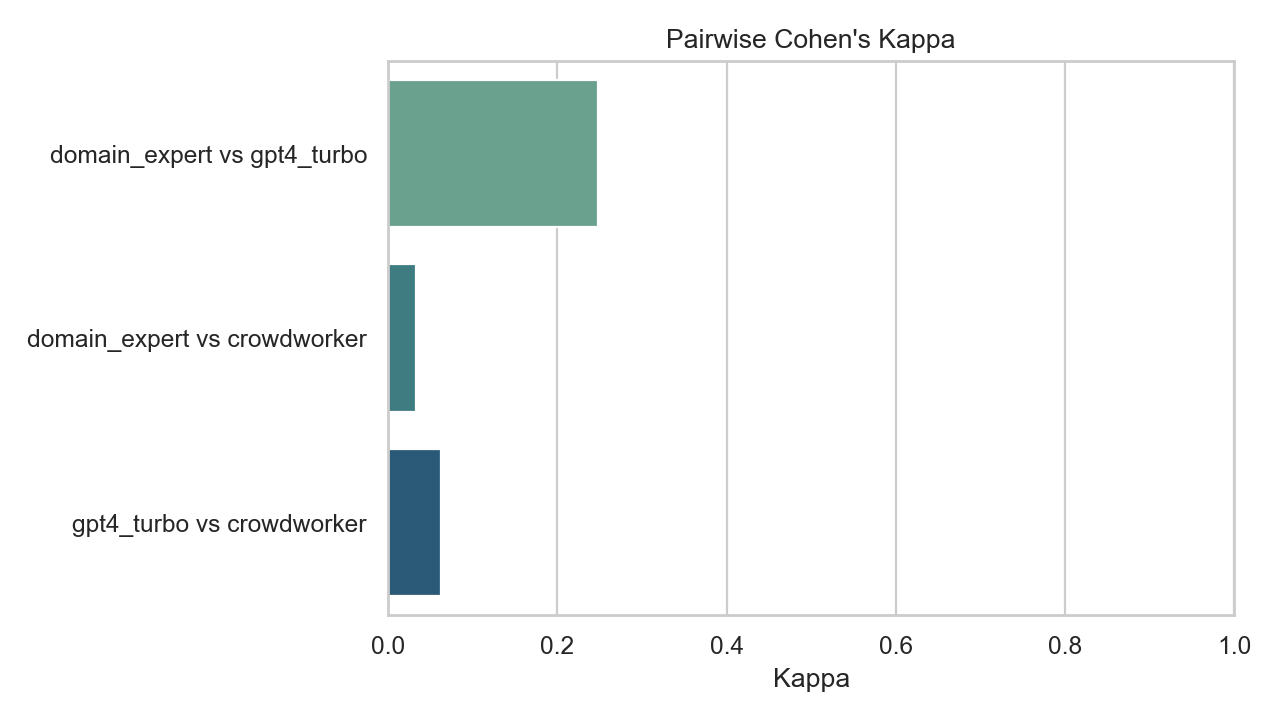
\includegraphics[width=0.82\textwidth]{uploads/implementation_agreement_kappa.png}
\caption{Pairwise Cohen's kappa for the three binary label sources.}
\label{fig:implementation-agreement-kappa}
\end{figure}

The kappa values show that the weak sources are noisy relative to domain experts. GPT-4-Turbo has stronger chance-adjusted agreement with domain expert labels than crowdworkers, but neither weak source is reliable enough to be treated as ground truth. This supports the decision to use weighted weak supervision with abstention.

\subsubsection{Weak-Supervision Results}

The weak-supervision step estimated nearly equal normalized reliability weights for the two weak sources:

\begin{itemize}
    \item GPT-4-Turbo weight: 0.499106.
    \item Crowdworker weight: 0.500894.
\end{itemize}

The weak-label acceptance summary is shown in Table \ref{tab:implementation-weak-labels}.

\begin{table}[H]
\centering
\small
\renewcommand{\arraystretch}{1.25}
\begin{tabular}{|l|r|}
\hline
\textbf{Weak-label metric} & \textbf{Value} \\
\hline
Candidate rows & 940 \\
\hline
Accepted rows & 648 \\
\hline
Accepted harmful rows & 493 \\
\hline
Accepted harmless rows & 155 \\
\hline
\end{tabular}
\caption{Weak-label acceptance summary.}
\label{tab:implementation-weak-labels}
\end{table}

Weak supervision adds a modest number of additional training rows. Because the accepted rows are restricted by confidence and leakage rules, the augmentation is conservative rather than simply merging all GPT and crowdworker labels.

\subsubsection{Pseudo-Labeling Results}

Pseudo-labeling was exercised on the corrected unlabeled pool. Table \ref{tab:implementation-pseudo-labels} shows the acceptance funnel.

\begin{table}[H]
\centering
\small
\renewcommand{\arraystretch}{1.25}
\begin{tabular}{|l|r|}
\hline
\textbf{Pseudo-label funnel metric} & \textbf{Value} \\
\hline
Rows with any text & 40401 \\
\hline
Rows after holdout exclusion & 40401 \\
\hline
Rows with at least 30 tokens & 35676 \\
\hline
Accepted pseudo-labels & 9254 \\
\hline
Accepted harmful pseudo-labels & 9253 \\
\hline
Accepted harmless pseudo-labels & 1 \\
\hline
Kept for final model & No \\
\hline
\end{tabular}
\caption{Pseudo-label acceptance funnel.}
\label{tab:implementation-pseudo-labels}
\end{table}

Although many pseudo-labels were accepted, they were almost entirely harmful. The pseudo-label model reduced validation macro-F1 compared with the weak-supervision model, so it was not selected as the final model. This is an important negative result: larger training data did not automatically produce a better classifier.

\subsubsection{Model Comparison}

The main binary test results are shown in Table \ref{tab:implementation-model-comparison}. All trained models beat the majority baseline on macro-F1. The weak-supervision model gives the best test macro-F1 among the three trained variants, while pseudo-labeling reduces macro-F1.

\begin{table}[H]
\centering
\scriptsize
\renewcommand{\arraystretch}{1.25}
\begin{tabularx}{\textwidth}{|>{\raggedright\arraybackslash}X|r|r|r|r|r|r|}
\hline
\textbf{Model} & \textbf{Macro-F1} & \textbf{Weighted F1} & \textbf{Precision} & \textbf{Recall} & \textbf{AUROC} & \textbf{PR-AUC} \\
\hline
Majority baseline & 0.4507 & 0.7397 & 0.8206 & 1.0000 & 0.5000 & 0.8206 \\
\hline
Expert only & 0.5701 & 0.7821 & 0.8400 & 0.9712 & 0.7442 & 0.9267 \\
\hline
Expert + weak supervision & 0.5740 & 0.7842 & 0.8408 & 0.9726 & 0.7443 & 0.9274 \\
\hline
Expert + weak supervision + pseudo-labeling & 0.5665 & 0.7809 & 0.8392 & 0.9726 & 0.7411 & 0.9276 \\
\hline
\end{tabularx}
\caption{Expert test split metrics for the majority baseline and trained model variants.}
\label{tab:implementation-model-comparison}
\end{table}

\begin{figure}[H]
\centering
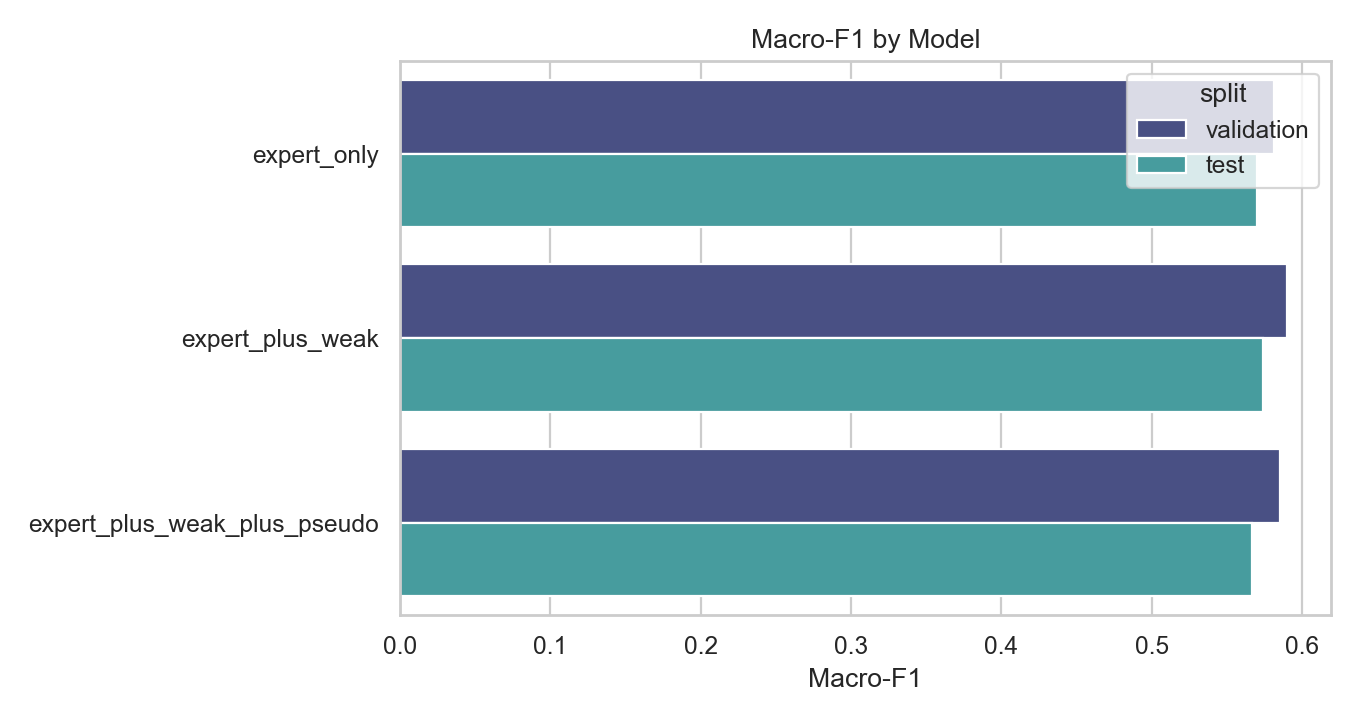
\includegraphics[width=0.82\textwidth]{uploads/implementation_model_macro_f1.png}
\caption{Macro-F1 comparison across trained model variants and data splits.}
\label{fig:implementation-model-macro-f1}
\end{figure}

The final selected model is the expert plus weak-supervision model. It improves expert test macro-F1 from 0.5701 to 0.5740 and slightly improves recall from 0.9712 to 0.9726. The improvement is modest, but it is consistent with the validation-based selection rule.

\subsubsection{Confusion Matrix Analysis}

The confusion matrices in Table \ref{tab:implementation-confusion-matrices} show the main error tradeoff. The final weak-supervision model reduces false negatives from 65 to 62 compared with the expert-only baseline and slightly increases true negatives from 76 to 78.

\begin{table}[H]
\centering
\small
\renewcommand{\arraystretch}{1.25}
\begin{tabular}{|l|r|r|r|r|}
\hline
\textbf{Model} & \textbf{TN} & \textbf{FP} & \textbf{FN} & \textbf{TP} \\
\hline
Expert only & 76 & 418 & 65 & 2194 \\
\hline
Expert + weak supervision & 78 & 416 & 62 & 2197 \\
\hline
Expert + weak supervision + pseudo-labeling & 73 & 421 & 62 & 2197 \\
\hline
\end{tabular}
\caption{Expert test split confusion matrices, flattened as TN, FP, FN, and TP.}
\label{tab:implementation-confusion-matrices}
\end{table}

The model achieves very high harmful-class recall, which is useful for moderation triage. However, the number of false positives remains high. This explains why macro-F1 is much lower than harmful-class recall and shows that threshold selection matters for practical use.

\subsubsection{Validation Threshold Sweep}

The default binary decision threshold is 0.5, but a threshold sweep was performed on the validation split to understand the precision-recall tradeoff. Table \ref{tab:implementation-threshold-sweep} reports the best validation thresholds by macro-F1.

\begin{table}[H]
\centering
\small
\renewcommand{\arraystretch}{1.25}
\begin{tabular}{|l|r|r|r|r|}
\hline
\textbf{Model} & \textbf{Threshold} & \textbf{Macro-F1} & \textbf{Precision} & \textbf{Recall} \\
\hline
Expert only & 0.70 & 0.6619 & 0.8771 & 0.8853 \\
\hline
Expert + weak supervision & 0.70 & 0.6605 & 0.8769 & 0.8835 \\
\hline
Expert + weak supervision + pseudo-labeling & 0.75 & 0.6574 & 0.8898 & 0.8264 \\
\hline
\end{tabular}
\caption{Best validation thresholds by macro-F1 for the trained model variants.}
\label{tab:implementation-threshold-sweep}
\end{table}

The threshold sweep shows that higher thresholds can improve macro-F1 by reducing false positives, but they also reduce harmful-class recall. A real moderation workflow could choose a threshold based on review capacity and the relative cost of false positives and false negatives.

\subsubsection{Strict Consensus Benchmark}

The strict consensus benchmark evaluates videos where all three label sources agree: \texttt{HHH} for harmful and \texttt{NNN} for harmless. This benchmark is expected to be easier because it focuses on less ambiguous examples.

\begin{table}[H]
\centering
\scriptsize
\renewcommand{\arraystretch}{1.25}
\begin{tabularx}{\textwidth}{|>{\raggedright\arraybackslash}X|r|r|r|r|r|r|}
\hline
\textbf{Model} & \textbf{Macro-F1} & \textbf{Weighted F1} & \textbf{Precision} & \textbf{Recall} & \textbf{AUROC} & \textbf{PR-AUC} \\
\hline
Expert only & 0.6732 & 0.8995 & 0.9254 & 0.9867 & 0.8597 & 0.9803 \\
\hline
Expert + weak supervision & 0.6845 & 0.9035 & 0.9266 & 0.9901 & 0.8647 & 0.9809 \\
\hline
Expert + weak supervision + pseudo-labeling & 0.6722 & 0.9002 & 0.9247 & 0.9901 & 0.8583 & 0.9800 \\
\hline
\end{tabularx}
\caption{Strict HHH/NNN consensus benchmark metrics.}
\label{tab:implementation-consensus-benchmark}
\end{table}

The weak-supervision model improves consensus macro-F1 from 0.6732 to 0.6845. This supports the conclusion that weak supervision improves robustness on clearer, high-agreement examples, even though the overall gain is small.

\subsubsection{Error Analysis}

The final model's errors were grouped into correct high-confidence predictions, false positives, false negatives, and missing-transcript cases. Table \ref{tab:implementation-error-examples} shows representative examples.

\begin{table}[H]
\centering
\scriptsize
\renewcommand{\arraystretch}{1.25}
\begin{tabularx}{\textwidth}{|p{2.8cm}|p{2.4cm}|r|r|r|X|}
\hline
\textbf{Case type} & \textbf{Video ID} & \textbf{Prob.} & \textbf{Pred.} & \textbf{True} & \textbf{Title} \\
\hline
Correct high-confidence & \texttt{QA28Ze6HBME} & 0.9967 & 1 & 1 & The MOST Insane Sh** I've EVER Witnessed !!! \\
\hline
False positive & \texttt{ZR5Wx1aTNXU} & 0.9812 & 1 & 0 & James Webb Telescope Discovers NEW 10th Planet Bigger Than Pluto \\
\hline
False negative & \texttt{OutB8gXxbO0} & 0.4951 & 0 & 1 & My Anorexia Recovery: Thinspo \\
\hline
Missing transcript & \texttt{C7lRtA83SQM} & 0.9903 & 1 & 1 & BIG LOST IN CASINO LAS VEGAS ROULETTE HOT BET TABLE HOT EXCLUSIVE 2023-04-08 \\
\hline
\end{tabularx}
\caption{Representative final-model prediction examples from the expert test split.}
\label{tab:implementation-error-examples}
\end{table}

The false positive example suggests that sensational wording can resemble harmful-content language even when the domain expert label is harmless. The false negative example shows the opposite risk: a harmful or sensitive topic may be framed in a recovery-oriented or ambiguous way, making the text signal harder to classify. Missing or noisy transcripts remain a key limitation for a text-first system.

\subsubsection{Demo API Verification}

The local demo API was verified against three practical requirements: empty inputs are rejected, repeated identical inputs produce deterministic outputs, and average prediction latency after model load remains under one second. The response format includes the binary harmful decision, harmful probability, risk band, and model version.

\begin{table}[H]
\centering
\small
\renewcommand{\arraystretch}{1.25}
\begin{tabularx}{\textwidth}{|>{\raggedright\arraybackslash}p{4.5cm}|>{\raggedright\arraybackslash}X|}
\hline
\textbf{API behavior} & \textbf{Verification result} \\
\hline
Reject empty title, description, and transcript & Passed \\
\hline
Return required fields in prediction response & Passed \\
\hline
Return deterministic output for repeated identical input & Passed \\
\hline
Average latency below one second after model load & Passed \\
\hline
\end{tabularx}
\caption{Demo API verification summary.}
\label{tab:implementation-api-verification}
\end{table}

This confirms that the final model can be used through a lightweight local interface after the batch training workflow is complete.

\subsubsection{Overall Result}

The final selected model is \texttt{expert\_plus\_weak}. It is selected because weak supervision improves validation and test macro-F1 relative to the expert-only baseline, while pseudo-labeling reduces validation macro-F1 and is therefore rejected by the fallback rule. The final test metrics are:

\begin{itemize}
    \item Macro-F1: 0.5740.
    \item Weighted F1: 0.7842.
    \item Precision: 0.8408.
    \item Recall: 0.9726.
    \item AUROC: 0.7443.
    \item PR-AUC: 0.9274.
\end{itemize}

The main conclusion is that the implemented pipeline successfully builds reproducible data layers, performs auditable label consolidation, compares supervised and weakly supervised models fairly, exercises pseudo-labeling, and exposes the selected binary classifier through a local API. Weak supervision provides a modest improvement, while pseudo-labeling is documented as a negative result under the validation-based selection rule.


\clearpage

\section{Tổng kết}

\subsection{Thảo luận}

Đề tài đã triển khai một pipeline hoàn chỉnh, ưu tiên văn bản, cho bài toán phát hiện video độc hại bằng giám sát yếu và gán nhãn giả. Đóng góp chính không chỉ nằm ở bộ phân loại cuối cùng, mà còn ở toàn bộ quy trình kỹ thuật xoay quanh mô hình: nhập dữ liệu không đồng nhất, làm sạch theo từng nguồn, hợp nhất văn bản chuẩn hóa, khả năng kiểm toán, chia tập tránh rò rỉ, phân tích đồng thuận, so sánh mô hình và suy luận cục bộ thông qua API minh họa.

\subsubsection{Những điểm hoạt động hiệu quả}

Thiết kế kỹ thuật dữ liệu hoạt động tốt với cấu trúc dữ liệu nhiều nhiễu của bộ dữ liệu. Mô hình ba tầng bronze, silver và gold giúp pipeline dễ phân tích hơn vì mỗi giai đoạn có một mục đích rõ ràng. Việc bảo toàn dữ liệu thô, chuẩn hóa lược đồ và hợp nhất dữ liệu sẵn sàng cho mô hình được tách riêng thay vì trộn lẫn với nhau. Sự tách biệt này quan trọng đối với các dự án nội dung độc hại vì những quyết định làm sạch dữ liệu nhỏ có thể trực tiếp làm thay đổi hành vi của mô hình.

Bảng wide chuẩn hóa cũng trở thành một hợp đồng mô hình hóa hữu ích. Bằng cách giữ một dòng cho mỗi mã định danh video và chọn các trường tiêu đề, mô tả, bản ghi lời nói dài nhất nhưng không rỗng, pipeline bảo toàn được phần văn bản giàu thông tin hơn khi cùng một video xuất hiện ở nhiều nguồn. Đồng thời, kiểm toán trùng lặp và hợp nhất giúp quá trình này có thể truy vết.

Phân tích đồng thuận cũng có giá trị đáng kể. Các giá trị kappa của Cohen đo được cho thấy nhãn của GPT-4-Turbo và crowdworker không hành xử như ground truth sạch. Điều này củng cố thiết kế giám sát yếu: các nguồn yếu có ích, nhưng cần được gán trọng số và lọc thay vì gộp trực tiếp vào tập huấn luyện.

Từ góc độ mô hình hóa, giám sát yếu đem lại một mức cải thiện nhỏ nhưng nhất quán so với mô hình nền chỉ dùng chuyên gia. Trên tập test chuyên gia, macro-F1 tăng từ 0.5701 lên 0.5740, và recall của lớp độc hại tăng từ 0.9712 lên 0.9726. Mức cải thiện này nhỏ, nhưng có ý nghĩa vì các nhãn yếu được chấp nhận một cách thận trọng và tập validation/test được bảo vệ khỏi rò rỉ dữ liệu.

\subsubsection{Những điểm chưa đạt hiệu quả như mong muốn}

Gán nhãn giả không cải thiện mô hình cuối cùng. Mặc dù tập chưa gán nhãn chứa nhiều dòng có văn bản và bước gán nhãn giả chấp nhận 9254 mẫu độ tin cậy cao, các nhãn được chấp nhận bị mất cân bằng nghiêm trọng: 9253 nhãn là độc hại và chỉ 1 nhãn là không độc hại. Sau khi huấn luyện lại, mô hình có nhãn giả làm giảm macro-F1 trên validation so với mô hình giám sát yếu. Theo quy tắc dự phòng của đề tài, mô hình có nhãn giả vì vậy không được chọn.

Kết quả âm này vẫn hữu ích. Nó cho thấy việc tăng số lượng dữ liệu huấn luyện không tự động có lợi khi các nhãn bổ sung do chính mô hình sinh ra. Gán nhãn giả có thể khuếch đại thiên lệch hiện có của mô hình, đặc biệt khi các mẫu được chấp nhận tập trung vào một lớp. Trong đề tài này, quy tắc lựa chọn dựa trên validation đã ngăn mô hình yếu hơn trở thành mô hình được triển khai.

Mô hình cuối cùng cũng có một đánh đổi precision-recall đáng chú ý. Mô hình đạt recall rất cao cho lớp độc hại, nhưng vẫn tạo ra nhiều false positive ở ngưỡng mặc định. Điều này có thể chấp nhận được đối với một prototype hướng đến phân loại ưu tiên, nơi việc bỏ sót nội dung độc hại có chi phí cao, nhưng cần điều chỉnh ngưỡng cẩn thận trước khi sử dụng trong một quy trình kiểm duyệt thực tế. Một nhóm rà soát có năng lực hạn chế có thể ưu tiên ngưỡng cao hơn để giảm false positive.

\subsubsection{Hạn chế}

Hạn chế thứ nhất là phạm vi dữ liệu. Hệ thống được thiết kế cho phát hiện video độc hại theo kiểu dữ liệu của các nền tảng phát trực tuyến, nhưng các thí nghiệm chỉ được đánh giá trên dữ liệu MetaHarm có nguồn gốc từ YouTube. Vì vậy, báo cáo không nên khẳng định mô hình đã được chứng minh có khả năng tổng quát hóa trên mọi nền tảng phát trực tuyến. Khẳng định phù hợp hơn là thiết kế pipeline có tính tổng quát và có thể được điều chỉnh cho các nền tảng khác nếu có các nguồn văn bản và nhãn tương đương.

Hạn chế thứ hai là phương thức dữ liệu. Mô hình hiện tại chỉ sử dụng tiêu đề, mô tả và bản ghi lời nói. Điều này giúp pipeline có khả năng tái lập và dễ chạy cục bộ hơn, nhưng cũng có nghĩa mô hình không thể hiểu nội dung thị giác, chữ xuất hiện trên màn hình, sắc thái âm thanh, hình nền hoặc ngữ cảnh cấp khung hình. Một số video độc hại có thể độc hại về mặt thị giác ngay cả khi tiêu đề và mô tả có vẻ không độc hại.

Hạn chế thứ ba là tính mơ hồ của nhãn. Chú thích nội dung độc hại mang tính chủ quan và phụ thuộc vào chính sách. Các giá trị đồng thuận thấp giữa các nguồn nhãn cho thấy ngay cả người chú thích và mô hình máy cũng có thể bất đồng đáng kể. Một số false positive và false negative do đó có thể phản ánh sự mơ hồ thực sự, không chỉ là lỗi đơn giản của mô hình.

Hạn chế thứ tư là sản phẩm hiện tại chỉ phân loại nhị phân. Hệ thống có thể xác định liệu một video có khả năng độc hại hay không, nhưng chưa giải thích loại tác hại cụ thể nào đang hiện diện. Dự đoán ở cấp nhóm tác hại sẽ hữu ích cho quy trình kiểm duyệt, nhưng cần một giai đoạn mô hình hóa và đánh giá bổ sung.

\subsubsection{Cân nhắc đạo đức và thực tiễn}

Phát hiện nội dung độc hại có thể ảnh hưởng đến mức độ hiển thị, thứ tự ưu tiên rà soát và kết quả kiểm duyệt. Một false positive có thể khiến nội dung không độc hại bị gắn cờ không công bằng, trong khi một false negative có thể để nội dung độc hại không bị phát hiện. Vì lý do này, mô hình nên được hiểu như một công cụ hỗ trợ quyết định thay vì một cơ chế thực thi tự động.

Hệ thống cũng cần được sử dụng với nhận thức về thiên lệch dữ liệu. Một mô hình được huấn luyện trên dữ liệu của một nền tảng có thể học các mẫu ngôn ngữ, quy ước chú thích hoặc giả định văn hóa đặc thù của nền tảng đó. Nếu hệ thống được điều chỉnh sang một nền tảng khác, nó cần được tái xác minh trên dữ liệu của nền tảng đó trước mọi hình thức sử dụng vận hành.

Cuối cùng, xác suất dự đoán không nên được xem là một lời giải thích đầy đủ. Đây là một tín hiệu xếp hạng hữu ích, nhưng người rà soát vẫn có thể cần ví dụ, đoạn văn bản được làm nổi bật, dự đoán loại tác hại hoặc các hình thức giải thích khác để hiểu vì sao một video bị gắn cờ.

\subsection{Kết luận}

Đề tài đã xây dựng thành công một pipeline phát hiện video độc hại ưu tiên văn bản, có khả năng tái lập, kết hợp giám sát yếu, gán nhãn giả, so sánh mô hình, báo cáo và API dự đoán cục bộ. Mô hình cuối cùng được chọn là \texttt{expert\_plus\_weak}, vì giám sát yếu cải thiện hành vi trên validation và test, trong khi gán nhãn giả làm giảm macro-F1 trên validation.

\begin{table}[H]
\centering
\small
\renewcommand{\arraystretch}{1.25}
\begin{tabular}{|l|r|}
\hline
\textbf{Chỉ số mô hình cuối cùng} & \textbf{Giá trị} \\
\hline
Mô hình được chọn & \texttt{expert\_plus\_weak} \\
\hline
Macro-F1 trên tập test chuyên gia & 0.5740 \\
\hline
Weighted F1 trên tập test chuyên gia & 0.7842 \\
\hline
Precision trên tập test chuyên gia & 0.8408 \\
\hline
Recall trên tập test chuyên gia & 0.9726 \\
\hline
AUROC trên tập test chuyên gia & 0.7443 \\
\hline
PR-AUC trên tập test chuyên gia & 0.9274 \\
\hline
Macro-F1 trên tập đồng thuận nghiêm ngặt & 0.6845 \\
\hline
\end{tabular}
\caption{Tóm tắt mô hình cuối cùng được chọn.}
\label{tab:summary-final-model}
\end{table}

Kết quả cho thấy giám sát yếu có thể đem lại một cải thiện nhỏ so với mô hình nền có giám sát chỉ dùng chuyên gia khi nhãn yếu được lọc cẩn thận và rò rỉ dữ liệu được kiểm soát. Thí nghiệm gán nhãn giả cho thấy một bài học khác: các mẫu chưa gán nhãn có độ tin cậy cao vẫn cần được xác minh bằng validation vì chúng có thể gây mất cân bằng lớp và làm giảm khả năng tổng quát hóa.

Nhìn chung, hệ thống hoàn thiện đáp ứng các mục tiêu chính của đề tài. Hệ thống tạo ra các tập dữ liệu đã xử lý có khả năng tái lập, ghi nhận vấn đề chất lượng dữ liệu, so sánh công bằng nhiều biến thể mô hình, ưu tiên macro-F1 và recall của lớp độc hại, báo cáo trung thực gán nhãn giả như một kết quả âm, đồng thời cung cấp mô hình được chọn thông qua một API cục bộ đơn giản.

\subsubsection{Hướng phát triển}

Một số hướng mở rộng có thể cải thiện hệ thống:

\begin{itemize}
    \item Triển khai sáu bộ phân loại one-vs-rest cho các nhóm tác hại \texttt{IH}, \texttt{HH}, \texttt{CB}, \texttt{ADD}, \texttt{SXL} và \texttt{PH}.
    \item Bổ sung điều chỉnh ngưỡng dựa trên chi phí kiểm duyệt thực tế và năng lực rà soát.
    \item Cải thiện hiệu chỉnh xác suất và lựa chọn nhãn giả để giảm mất cân bằng lớp.
    \item Khảo sát các mô hình văn bản mạnh hơn, chẳng hạn các bộ mã hóa dựa trên transformer, nếu tài nguyên tính toán cho phép.
    \item Bổ sung tín hiệu đa phương thức như ảnh thu nhỏ, khung hình được lấy mẫu hoặc đặc trưng suy ra từ âm thanh sau khi pipeline văn bản đã ổn định.
    \item Đánh giá pipeline trên các bộ dữ liệu ngoài YouTube hoặc đa nền tảng để kiểm tra khả năng tổng quát hóa trực tiếp hơn.
    \item Bổ sung các đặc trưng giải thích, chẳng hạn làm nổi bật các thuật ngữ quan trọng trong tiêu đề, mô tả hoặc bản ghi lời nói cho người rà soát.
    \item Cải thiện nhật ký chạy container và xác minh thực thi trên thêm các kiến trúc phần cứng.
\end{itemize}

Các hướng phát triển này có thể đưa đề tài từ một prototype xử lý theo lô cục bộ vững chắc tiến gần hơn tới một nền tảng nghiên cứu hoàn chỉnh cho phát hiện video độc hại.


\clearpage

\begin{thebibliography}{80}
\bibitem{ref1} Tác giả, \textit{Tên tài liệu}, Nhà xuất bản hoặc nguồn công bố, Năm.
\end{thebibliography}


\end{document}
